\documentclass[1p]{elsarticle_modified}
%\bibliographystyle{elsarticle-num}

%\usepackage[colorlinks]{hyperref}
%\usepackage{abbrmath_seonhwa} %\Abb, \Ascr, \Acal ,\Abf, \Afrak
\usepackage{amsfonts}
\usepackage{amssymb}
\usepackage{amsmath}
\usepackage{amsthm}
\usepackage{scalefnt}
\usepackage{amsbsy}
\usepackage{kotex}
\usepackage{caption}
\usepackage{subfig}
\usepackage{color}
\usepackage{graphicx}
\usepackage{xcolor} %% white, black, red, green, blue, cyan, magenta, yellow
\usepackage{float}
\usepackage{setspace}
\usepackage{hyperref}

\usepackage{tikz}
\usetikzlibrary{arrows}

\usepackage{multirow}
\usepackage{array} % fixed length table
\usepackage{hhline}

%%%%%%%%%%%%%%%%%%%%%
\makeatletter
\renewcommand*\env@matrix[1][\arraystretch]{%
	\edef\arraystretch{#1}%
	\hskip -\arraycolsep
	\let\@ifnextchar\new@ifnextchar
	\array{*\c@MaxMatrixCols c}}
\makeatother %https://tex.stackexchange.com/questions/14071/how-can-i-increase-the-line-spacing-in-a-matrix
%%%%%%%%%%%%%%%

\usepackage[normalem]{ulem}

\newcommand{\msout}[1]{\ifmmode\text{\sout{\ensuremath{#1}}}\else\sout{#1}\fi}
%SOURCE: \msout is \stkout macro in https://tex.stackexchange.com/questions/20609/strikeout-in-math-mode

\newcommand{\cancel}[1]{
	\ifmmode
	{\color{red}\msout{#1}}
	\else
	{\color{red}\sout{#1}}
	\fi
}

\newcommand{\add}[1]{
	{\color{blue}\uwave{#1}}
}

\newcommand{\replace}[2]{
	\ifmmode
	{\color{red}\msout{#1}}{\color{blue}\uwave{#2}}
	\else
	{\color{red}\sout{#1}}{\color{blue}\uwave{#2}}
	\fi
}

\newcommand{\Sol}{\mathcal{S}} %segment
\newcommand{\D}{D} %diagram
\newcommand{\A}{\mathcal{A}} %arc


%%%%%%%%%%%%%%%%%%%%%%%%%%%%%5 test

\def\sl{\operatorname{\textup{SL}}(2,\Cbb)}
\def\psl{\operatorname{\textup{PSL}}(2,\Cbb)}
\def\quan{\mkern 1mu \triangleright \mkern 1mu}

\theoremstyle{definition}
\newtheorem{thm}{Theorem}[section]
\newtheorem{prop}[thm]{Proposition}
\newtheorem{lem}[thm]{Lemma}
\newtheorem{ques}[thm]{Question}
\newtheorem{cor}[thm]{Corollary}
\newtheorem{defn}[thm]{Definition}
\newtheorem{exam}[thm]{Example}
\newtheorem{rmk}[thm]{Remark}
\newtheorem{alg}[thm]{Algorithm}

\newcommand{\I}{\sqrt{-1}}
\begin{document}

%\begin{frontmatter}
%
%\title{Boundary parabolic representations of knots up to 8 crossings}
%
%%% Group authors per affiliation:
%\author{Yunhi Cho} 
%\address{Department of Mathematics, University of Seoul, Seoul, Korea}
%\ead{yhcho@uos.ac.kr}
%
%
%\author{Seonhwa Kim} %\fnref{s_kim}}
%\address{Center for Geometry and Physics, Institute for Basic Science, Pohang, 37673, Korea}
%\ead{ryeona17@ibs.re.kr}
%
%\author{Hyuk Kim}
%\address{Department of Mathematical Sciences, Seoul National University, Seoul 08826, Korea}
%\ead{hyukkim@snu.ac.kr}
%
%\author{Seokbeom Yoon}
%\address{Department of Mathematical Sciences, Seoul National University, Seoul, 08826,  Korea}
%\ead{sbyoon15@snu.ac.kr}
%
%\begin{abstract}
%We find all boundary parabolic representation of knots up to 8 crossings.
%
%\end{abstract}
%\begin{keyword}
%    \MSC[2010] 57M25 
%\end{keyword}
%
%\end{frontmatter}

%\linenumbers
%\tableofcontents
%
\newcommand\colored[1]{\textcolor{white}{\rule[-0.35ex]{0.8em}{1.4ex}}\kern-0.8em\color{red} #1}%
%\newcommand\colored[1]{\textcolor{white}{ #1}\kern-2.17ex	\textcolor{white}{ #1}\kern-1.81ex	\textcolor{white}{ #1}\kern-2.15ex\color{red}#1	}

{\Large $\underline{12a_{0653}~(K12a_{0653})}$}

\setlength{\tabcolsep}{10pt}
\renewcommand{\arraystretch}{1.6}
\vspace{1cm}\begin{tabular}{m{100pt}>{\centering\arraybackslash}m{274pt}}
\multirow{5}{120pt}{
	\centering
	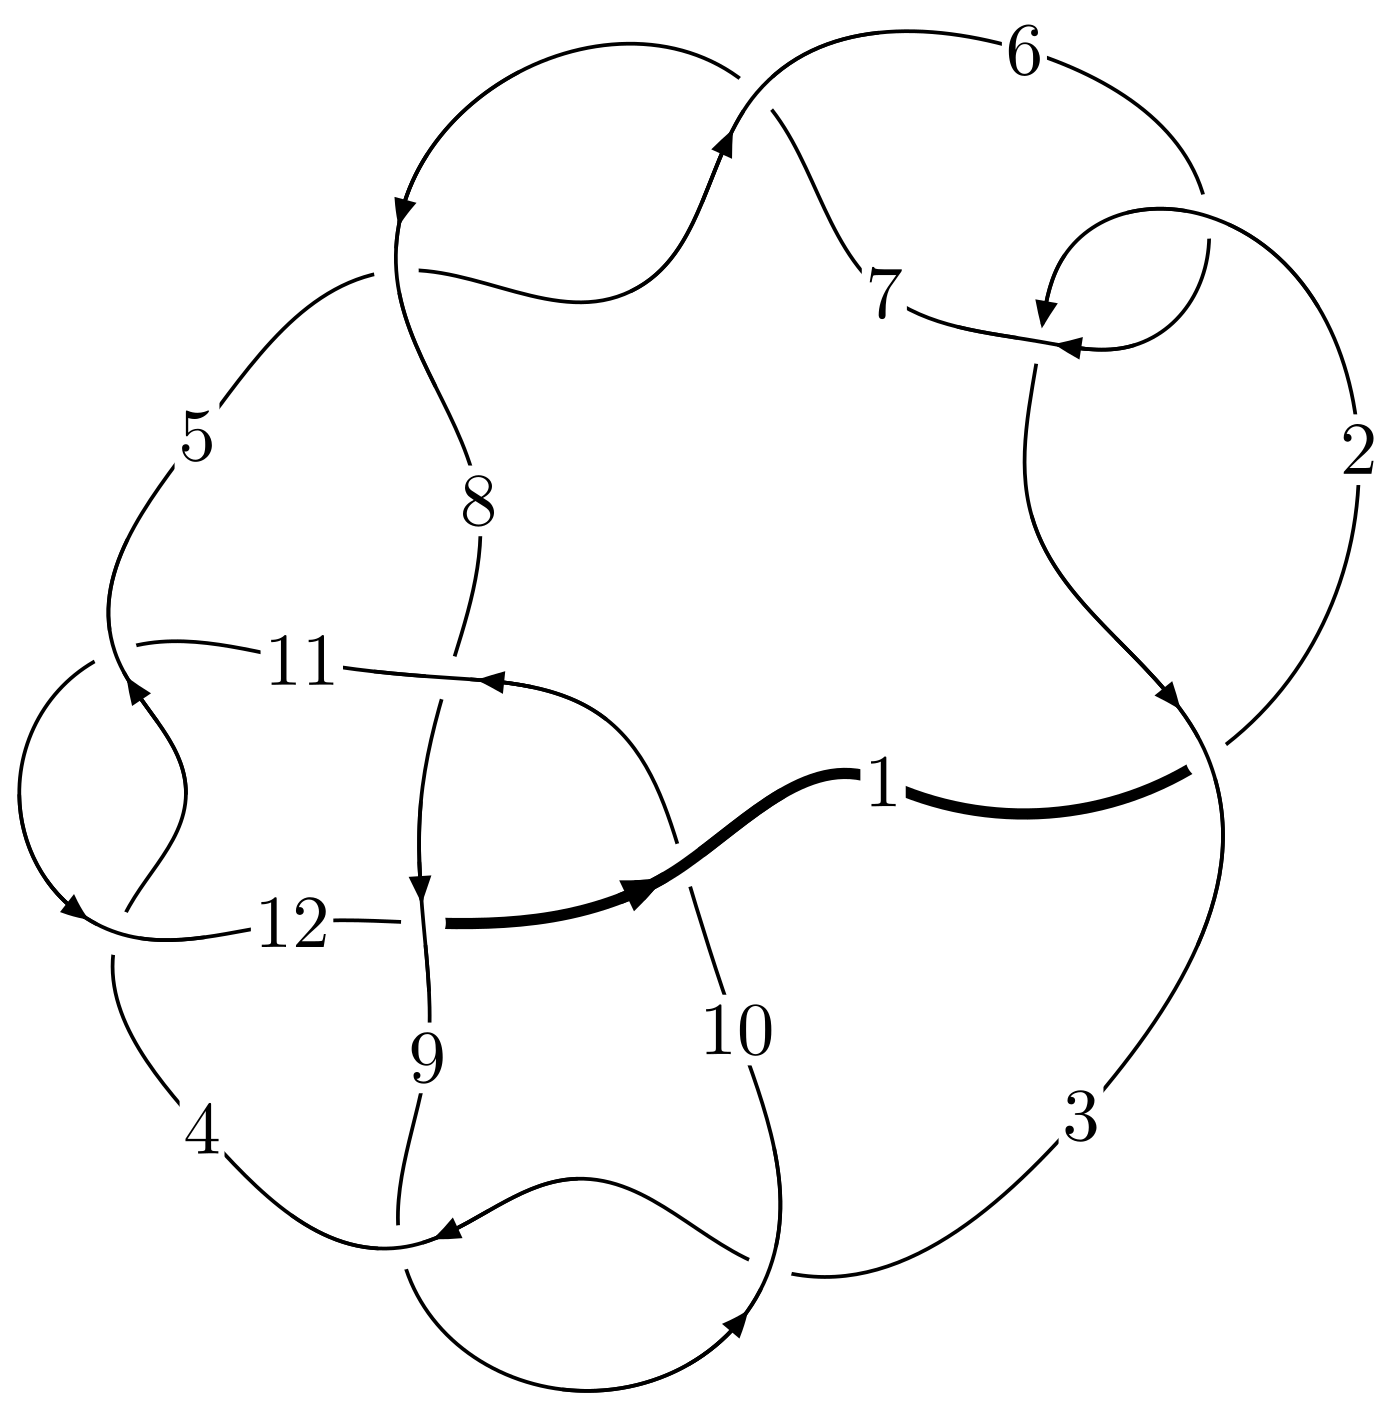
\includegraphics[width=112pt]{../../../GIT/diagram.site/Diagrams/png/1454_12a_0653.png}\\
\ \ \ A knot diagram\footnotemark}&
\allowdisplaybreaks
\textbf{Linearized knot diagam} \\
\cline{2-2}
 &
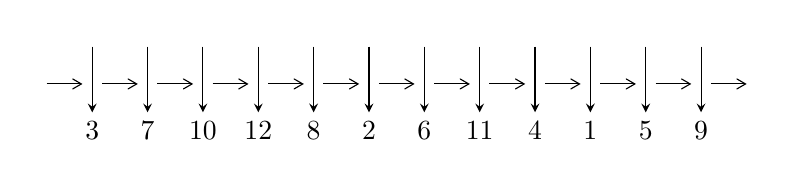
\begin{tikzpicture}[x=20pt, y=17pt]
	% nodes
	\node (C0) at (0, 0) {};
	\node (C1) at (1, 0) {};
	\node (C1U) at (1, +1) {};
	\node (C1D) at (1, -1) {3};

	\node (C2) at (2, 0) {};
	\node (C2U) at (2, +1) {};
	\node (C2D) at (2, -1) {7};

	\node (C3) at (3, 0) {};
	\node (C3U) at (3, +1) {};
	\node (C3D) at (3, -1) {10};

	\node (C4) at (4, 0) {};
	\node (C4U) at (4, +1) {};
	\node (C4D) at (4, -1) {12};

	\node (C5) at (5, 0) {};
	\node (C5U) at (5, +1) {};
	\node (C5D) at (5, -1) {8};

	\node (C6) at (6, 0) {};
	\node (C6U) at (6, +1) {};
	\node (C6D) at (6, -1) {2};

	\node (C7) at (7, 0) {};
	\node (C7U) at (7, +1) {};
	\node (C7D) at (7, -1) {6};

	\node (C8) at (8, 0) {};
	\node (C8U) at (8, +1) {};
	\node (C8D) at (8, -1) {11};

	\node (C9) at (9, 0) {};
	\node (C9U) at (9, +1) {};
	\node (C9D) at (9, -1) {4};

	\node (C10) at (10, 0) {};
	\node (C10U) at (10, +1) {};
	\node (C10D) at (10, -1) {1};

	\node (C11) at (11, 0) {};
	\node (C11U) at (11, +1) {};
	\node (C11D) at (11, -1) {5};

	\node (C12) at (12, 0) {};
	\node (C12U) at (12, +1) {};
	\node (C12D) at (12, -1) {9};
	\node (C13) at (13, 0) {};

	% arrows
	\draw[->,>={angle 60}]
	(C0) edge (C1) (C1) edge (C2) (C2) edge (C3) (C3) edge (C4) (C4) edge (C5) (C5) edge (C6) (C6) edge (C7) (C7) edge (C8) (C8) edge (C9) (C9) edge (C10) (C10) edge (C11) (C11) edge (C12) (C12) edge (C13) ;	\draw[->,>=stealth]
	(C1U) edge (C1D) (C2U) edge (C2D) (C3U) edge (C3D) (C4U) edge (C4D) (C5U) edge (C5D) (C6U) edge (C6D) (C7U) edge (C7D) (C8U) edge (C8D) (C9U) edge (C9D) (C10U) edge (C10D) (C11U) edge (C11D) (C12U) edge (C12D) ;
	\end{tikzpicture} \\
\hhline{~~} \\& 
\textbf{Solving Sequence} \\ \cline{2-2} 
 &
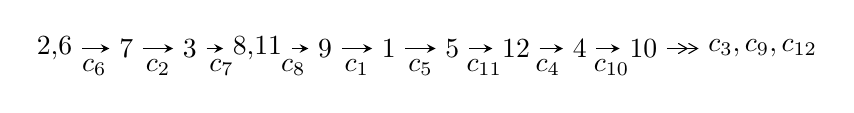
\begin{tikzpicture}[x=23pt, y=7pt]
	% node
	\node (A0) at (-1/8, 0) {2,6};
	\node (A1) at (1, 0) {7};
	\node (A2) at (2, 0) {3};
	\node (A3) at (49/16, 0) {8,11};
	\node (A4) at (33/8, 0) {9};
	\node (A5) at (41/8, 0) {1};
	\node (A6) at (49/8, 0) {5};
	\node (A7) at (57/8, 0) {12};
	\node (A8) at (65/8, 0) {4};
	\node (A9) at (73/8, 0) {10};
	\node (C1) at (1/2, -1) {$c_{6}$};
	\node (C2) at (3/2, -1) {$c_{2}$};
	\node (C3) at (5/2, -1) {$c_{7}$};
	\node (C4) at (29/8, -1) {$c_{8}$};
	\node (C5) at (37/8, -1) {$c_{1}$};
	\node (C6) at (45/8, -1) {$c_{5}$};
	\node (C7) at (53/8, -1) {$c_{11}$};
	\node (C8) at (61/8, -1) {$c_{4}$};
	\node (C9) at (69/8, -1) {$c_{10}$};
	\node (A10) at (11, 0) {$c_{3},c_{9},c_{12}$};

	% edge
	\draw[->,>=stealth]	
	(A0) edge (A1) (A1) edge (A2) (A2) edge (A3) (A3) edge (A4) (A4) edge (A5) (A5) edge (A6) (A6) edge (A7) (A7) edge (A8) (A8) edge (A9) ;
	\draw[->>,>={angle 60}]	
	(A9) edge (A10);
\end{tikzpicture} \\ 

\end{tabular} \\

\footnotetext{
The image of knot diagram is generated by the software ``\textbf{Draw programme}" developed by Andrew Bartholomew(\url{http://www.layer8.co.uk/maths/draw/index.htm\#Running-draw}), where we modified some parts for our purpose(\url{https://github.com/CATsTAILs/LinksPainter}).
}\phantom \\ \newline 
\centering \textbf{Ideals for irreducible components\footnotemark of $X_{\text{par}}$} 
 
\begin{align*}
I^u_{1}&=\langle 
23 u^{32}-20 u^{31}+\cdots+2 b+192,\;-83 u^{32}+367 u^{31}+\cdots+2 a+53,\;u^{33}-6 u^{32}+\cdots+2 u+4\rangle \\
I^u_{2}&=\langle 
3369103813 u^{13} a^3+32822425576 u^{13} a^2+\cdots+472218636585 a+522982296989,\\
\phantom{I^u_{2}}&\phantom{= \langle  }u^{13} a^3+8 u^{13} a^2+\cdots+22 a+15,\\
\phantom{I^u_{2}}&\phantom{= \langle  }u^{14}+u^{13}- u^{12}-2 u^{11}+4 u^{10}+5 u^9-3 u^8-6 u^7+4 u^6+6 u^5-2 u^4-2 u^3+2 u^2+u-1\rangle \\
I^u_{3}&=\langle 
u^{16}+u^{15}+\cdots+b-1,\\
\phantom{I^u_{3}}&\phantom{= \langle  }u^{16}+u^{15}- u^{14}-3 u^{13}+4 u^{12}+7 u^{11}-2 u^{10}-12 u^9+2 u^8+12 u^7+4 u^6-10 u^5-4 u^4+3 u^3+6 u^2+a-1,\\
\phantom{I^u_{3}}&\phantom{= \langle  }u^{17}+u^{16}-2 u^{15}-3 u^{14}+6 u^{13}+8 u^{12}-8 u^{11}-14 u^{10}+10 u^9+18 u^8-7 u^7-17 u^6+4 u^5+11 u^4-4 u^2+1\rangle \\
\\
\end{align*}
\raggedright * 3 irreducible components of $\dim_{\mathbb{C}}=0$, with total 106 representations.\\
\footnotetext{All coefficients of polynomials are rational numbers. But the coefficients are sometimes approximated in decimal forms when there is not enough margin.}
\newpage
\renewcommand{\arraystretch}{1}
\centering \section*{I. $I^u_{1}= \langle 23 u^{32}-20 u^{31}+\cdots+2 b+192,\;-83 u^{32}+367 u^{31}+\cdots+2 a+53,\;u^{33}-6 u^{32}+\cdots+2 u+4 \rangle$}
\flushleft \textbf{(i) Arc colorings}\\
\begin{tabular}{m{7pt} m{180pt} m{7pt} m{180pt} }
\flushright $a_{2}=$&$\begin{pmatrix}0\\u\end{pmatrix}$ \\
\flushright $a_{6}=$&$\begin{pmatrix}1\\0\end{pmatrix}$ \\
\flushright $a_{7}=$&$\begin{pmatrix}1\\u^2\end{pmatrix}$ \\
\flushright $a_{3}=$&$\begin{pmatrix}- u\\- u^3+u\end{pmatrix}$ \\
\flushright $a_{8}=$&$\begin{pmatrix}- u^2+1\\u^2\end{pmatrix}$ \\
\flushright $a_{11}=$&$\begin{pmatrix}\frac{83}{2} u^{32}-\frac{367}{2} u^{31}+\cdots+65 u-\frac{53}{2}\\-\frac{23}{2} u^{32}+10 u^{31}+\cdots-\frac{375}{2} u-96\end{pmatrix}$ \\
\flushright $a_{9}=$&$\begin{pmatrix}-\frac{45}{4} u^{32}+49 u^{31}+\cdots-\frac{115}{4} u+4\\\frac{5}{2} u^{32}-32 u^{30}+\cdots+\frac{113}{2} u+29\end{pmatrix}$ \\
\flushright $a_{1}=$&$\begin{pmatrix}u^3\\u^5- u^3+u\end{pmatrix}$ \\
\flushright $a_{5}=$&$\begin{pmatrix}u^4- u^2+1\\- u^4\end{pmatrix}$ \\
\flushright $a_{12}=$&$\begin{pmatrix}3 u^{32}-\frac{19}{2} u^{31}+\cdots+\frac{61}{2} u+\frac{19}{2}\\\frac{7}{2} u^{32}-20 u^{31}+\cdots-\frac{59}{2} u-20\end{pmatrix}$ \\
\flushright $a_{4}=$&$\begin{pmatrix}\frac{5}{4} u^{32}-3 u^{31}+\cdots+\frac{11}{4} u+2\\\frac{3}{2} u^{32}-12 u^{31}+\cdots-\frac{29}{2} u-11\end{pmatrix}$ \\
\flushright $a_{10}=$&$\begin{pmatrix}\frac{9}{2} u^{32}-\frac{43}{2} u^{31}+\cdots+3 u-\frac{13}{2}\\-\frac{19}{2} u^{32}+48 u^{31}+\cdots+\frac{47}{2} u+26\end{pmatrix}$\\&\end{tabular}
\flushleft \textbf{(ii) Obstruction class $= -1$}\\~\\
\flushleft \textbf{(iii) Cusp Shapes $= -25 u^{32}+137 u^{31}-250 u^{30}-48 u^{29}+729 u^{28}-349 u^{27}-1766 u^{26}+2220 u^{25}+1732 u^{24}-3935 u^{23}-1941 u^{22}+6635 u^{21}+458 u^{20}-6613 u^{19}-1876 u^{18}+8144 u^{17}+1987 u^{16}-6981 u^{15}-4913 u^{14}+8258 u^{13}+3726 u^{12}-5186 u^{11}-4612 u^{10}+3551 u^9+3476 u^8-959 u^7-3182 u^6+648 u^5+1495 u^4-98 u^3-504 u^2+14 u+46$}\\~\\
\newpage\renewcommand{\arraystretch}{1}
\flushleft \textbf{(iv) u-Polynomials at the component}\newline \\
\begin{tabular}{m{50pt}|m{274pt}}
Crossings & \hspace{64pt}u-Polynomials at each crossing \\
\hline $$\begin{aligned}c_{1},c_{5},c_{7}\end{aligned}$$&$\begin{aligned}
&u^{33}+8 u^{32}+\cdots+220 u+16
\end{aligned}$\\
\hline $$\begin{aligned}c_{2},c_{6}\end{aligned}$$&$\begin{aligned}
&u^{33}-6 u^{32}+\cdots+2 u+4
\end{aligned}$\\
\hline $$\begin{aligned}c_{3},c_{4},c_{9}\\c_{11}\end{aligned}$$&$\begin{aligned}
&u^{33}+15 u^{31}+\cdots+u+1
\end{aligned}$\\
\hline $$\begin{aligned}c_{8},c_{10}\end{aligned}$$&$\begin{aligned}
&u^{33}+3 u^{32}+\cdots+u+1
\end{aligned}$\\
\hline $$\begin{aligned}c_{12}\end{aligned}$$&$\begin{aligned}
&u^{33}+32 u^{32}+\cdots+286720 u+16384
\end{aligned}$\\
\hline
\end{tabular}\\~\\
\newpage\renewcommand{\arraystretch}{1}
\flushleft \textbf{(v) Riley Polynomials at the component}\newline \\
\begin{tabular}{m{50pt}|m{274pt}}
Crossings & \hspace{64pt}Riley Polynomials at each crossing \\
\hline $$\begin{aligned}c_{1},c_{5},c_{7}\end{aligned}$$&$\begin{aligned}
&y^{33}+36 y^{32}+\cdots+6256 y-256
\end{aligned}$\\
\hline $$\begin{aligned}c_{2},c_{6}\end{aligned}$$&$\begin{aligned}
&y^{33}-8 y^{32}+\cdots+220 y-16
\end{aligned}$\\
\hline $$\begin{aligned}c_{3},c_{4},c_{9}\\c_{11}\end{aligned}$$&$\begin{aligned}
&y^{33}+30 y^{32}+\cdots+5 y-1
\end{aligned}$\\
\hline $$\begin{aligned}c_{8},c_{10}\end{aligned}$$&$\begin{aligned}
&y^{33}+17 y^{32}+\cdots+63 y-1
\end{aligned}$\\
\hline $$\begin{aligned}c_{12}\end{aligned}$$&$\begin{aligned}
&y^{33}+2 y^{32}+\cdots+4630511616 y-268435456
\end{aligned}$\\
\hline
\end{tabular}\\~\\
\newpage\flushleft \textbf{(vi) Complex Volumes and Cusp Shapes}
$$\begin{array}{c|c|c}  
\text{Solutions to }I^u_{1}& \I (\text{vol} + \sqrt{-1}CS) & \text{Cusp shape}\\
 \hline 
\begin{aligned}
u &= \phantom{-}0.838398 + 0.613102 I \\
a &= -0.366122 + 0.442209 I \\
b &= \phantom{-}0.003736 - 0.378058 I\end{aligned}
 & \phantom{-}1.70782 - 2.40859 I & -4.73211 + 2.63884 I \\ \hline\begin{aligned}
u &= \phantom{-}0.838398 - 0.613102 I \\
a &= -0.366122 - 0.442209 I \\
b &= \phantom{-}0.003736 + 0.378058 I\end{aligned}
 & \phantom{-}1.70782 + 2.40859 I & -4.73211 - 2.63884 I \\ \hline\begin{aligned}
u &= -0.415165 + 0.823365 I \\
a &= -0.272267 + 0.601963 I \\
b &= \phantom{-}0.931790 + 0.355896 I\end{aligned}
 & \phantom{-}9.11306 - 7.42411 I & -3.38968 + 4.20871 I \\ \hline\begin{aligned}
u &= -0.415165 - 0.823365 I \\
a &= -0.272267 - 0.601963 I \\
b &= \phantom{-}0.931790 - 0.355896 I\end{aligned}
 & \phantom{-}9.11306 + 7.42411 I & -3.38968 - 4.20871 I \\ \hline\begin{aligned}
u &= -0.814655 + 0.420904 I \\
a &= -0.014524 + 0.720997 I \\
b &= \phantom{-}0.779019 + 0.954203 I\end{aligned}
 & -1.41171 + 3.25911 I & -15.5699 - 6.2232 I \\ \hline\begin{aligned}
u &= -0.814655 - 0.420904 I \\
a &= -0.014524 - 0.720997 I \\
b &= \phantom{-}0.779019 - 0.954203 I\end{aligned}
 & -1.41171 - 3.25911 I & -15.5699 + 6.2232 I \\ \hline\begin{aligned}
u &= -0.277153 + 0.867734 I \\
a &= \phantom{-}0.509978 - 0.137733 I \\
b &= -0.389242 - 0.632865 I\end{aligned}
 & \phantom{-}8.34160 + 3.38775 I & -0.87656 - 3.53440 I \\ \hline\begin{aligned}
u &= -0.277153 - 0.867734 I \\
a &= \phantom{-}0.509978 + 0.137733 I \\
b &= -0.389242 + 0.632865 I\end{aligned}
 & \phantom{-}8.34160 - 3.38775 I & -0.87656 + 3.53440 I \\ \hline\begin{aligned}
u &= \phantom{-}1.100190 + 0.089830 I \\
a &= -0.481622 - 0.649769 I \\
b &= \phantom{-}0.0208635 - 0.1183110 I\end{aligned}
 & \phantom{-}3.28828 - 5.97548 I & -8.94862 + 7.09482 I \\ \hline\begin{aligned}
u &= \phantom{-}1.100190 - 0.089830 I \\
a &= -0.481622 + 0.649769 I \\
b &= \phantom{-}0.0208635 + 0.1183110 I\end{aligned}
 & \phantom{-}3.28828 + 5.97548 I & -8.94862 - 7.09482 I\\
 \hline 
 \end{array}$$\newpage$$\begin{array}{c|c|c}  
\text{Solutions to }I^u_{1}& \I (\text{vol} + \sqrt{-1}CS) & \text{Cusp shape}\\
 \hline 
\begin{aligned}
u &= -0.863288 + 0.745766 I \\
a &= -0.337012 + 0.105923 I \\
b &= -0.139284 + 0.796748 I\end{aligned}
 & \phantom{-}1.75606 + 2.81515 I & -5.07945 - 3.99725 I \\ \hline\begin{aligned}
u &= -0.863288 - 0.745766 I \\
a &= -0.337012 - 0.105923 I \\
b &= -0.139284 - 0.796748 I\end{aligned}
 & \phantom{-}1.75606 - 2.81515 I & -5.07945 + 3.99725 I \\ \hline\begin{aligned}
u &= -1.021670 + 0.530532 I \\
a &= -0.224206 - 0.440345 I \\
b &= -1.110970 - 0.423583 I\end{aligned}
 & \phantom{-}7.0965 + 12.3235 I & -7.48212 - 9.31831 I \\ \hline\begin{aligned}
u &= -1.021670 - 0.530532 I \\
a &= -0.224206 + 0.440345 I \\
b &= -1.110970 + 0.423583 I\end{aligned}
 & \phantom{-}7.0965 - 12.3235 I & -7.48212 + 9.31831 I \\ \hline\begin{aligned}
u &= -1.125530 + 0.460328 I \\
a &= \phantom{-}0.246731 + 0.066023 I \\
b &= \phantom{-}0.636793 - 0.225287 I\end{aligned}
 & \phantom{-}5.49810 + 1.42945 I & -1.94384 - 1.59393 I \\ \hline\begin{aligned}
u &= -1.125530 - 0.460328 I \\
a &= \phantom{-}0.246731 - 0.066023 I \\
b &= \phantom{-}0.636793 + 0.225287 I\end{aligned}
 & \phantom{-}5.49810 - 1.42945 I & -1.94384 + 1.59393 I \\ \hline\begin{aligned}
u &= \phantom{-}0.755893 + 0.131338 I \\
a &= \phantom{-}1.56947 - 0.67478 I \\
b &= -0.271312 + 0.241644 I\end{aligned}
 & -2.89891 - 0.34125 I & -18.0890 + 12.2689 I \\ \hline\begin{aligned}
u &= \phantom{-}0.755893 - 0.131338 I \\
a &= \phantom{-}1.56947 + 0.67478 I \\
b &= -0.271312 - 0.241644 I\end{aligned}
 & -2.89891 + 0.34125 I & -18.0890 - 12.2689 I \\ \hline\begin{aligned}
u &= \phantom{-}0.902285 + 0.867527 I \\
a &= \phantom{-}1.60945 + 1.85954 I \\
b &= -2.65111 - 0.44007 I\end{aligned}
 & \phantom{-}6.37334 - 0.89739 I & -9.49648 - 0.54814 I \\ \hline\begin{aligned}
u &= \phantom{-}0.902285 - 0.867527 I \\
a &= \phantom{-}1.60945 - 1.85954 I \\
b &= -2.65111 + 0.44007 I\end{aligned}
 & \phantom{-}6.37334 + 0.89739 I & -9.49648 + 0.54814 I\\
 \hline 
 \end{array}$$\newpage$$\begin{array}{c|c|c}  
\text{Solutions to }I^u_{1}& \I (\text{vol} + \sqrt{-1}CS) & \text{Cusp shape}\\
 \hline 
\begin{aligned}
u &= \phantom{-}0.929251 + 0.857665 I \\
a &= -2.32439 - 1.06449 I \\
b &= \phantom{-}2.64641 - 0.85846 I\end{aligned}
 & \phantom{-}6.28919 - 5.49945 I & -9.75207 + 5.34386 I \\ \hline\begin{aligned}
u &= \phantom{-}0.929251 - 0.857665 I \\
a &= -2.32439 + 1.06449 I \\
b &= \phantom{-}2.64641 + 0.85846 I\end{aligned}
 & \phantom{-}6.28919 + 5.49945 I & -9.75207 - 5.34386 I \\ \hline\begin{aligned}
u &= \phantom{-}0.863589 + 0.938538 I \\
a &= -1.84094 - 1.56412 I \\
b &= \phantom{-}2.90596 + 0.30561 I\end{aligned}
 & \phantom{-}17.0337 + 9.7572 I & -4.21655 - 3.66521 I \\ \hline\begin{aligned}
u &= \phantom{-}0.863589 - 0.938538 I \\
a &= -1.84094 + 1.56412 I \\
b &= \phantom{-}2.90596 - 0.30561 I\end{aligned}
 & \phantom{-}17.0337 - 9.7572 I & -4.21655 + 3.66521 I \\ \hline\begin{aligned}
u &= \phantom{-}0.844668 + 0.965107 I \\
a &= \phantom{-}1.26522 + 0.67302 I \\
b &= -1.79222 + 0.12655 I\end{aligned}
 & \phantom{-}15.6006 + 0.0709 I & -2.15054 + 0. I\phantom{ +0.000000I} \\ \hline\begin{aligned}
u &= \phantom{-}0.844668 - 0.965107 I \\
a &= \phantom{-}1.26522 - 0.67302 I \\
b &= -1.79222 - 0.12655 I\end{aligned}
 & \phantom{-}15.6006 - 0.0709 I & -2.15054 + 0. I\phantom{ +0.000000I} \\ \hline\begin{aligned}
u &= \phantom{-}0.995894 + 0.870348 I \\
a &= \phantom{-}2.13894 + 1.52075 I \\
b &= -2.94172 + 0.68814 I\end{aligned}
 & \phantom{-}16.6040 - 16.4117 I & -4.91951 + 8.23114 I \\ \hline\begin{aligned}
u &= \phantom{-}0.995894 - 0.870348 I \\
a &= \phantom{-}2.13894 - 1.52075 I \\
b &= -2.94172 - 0.68814 I\end{aligned}
 & \phantom{-}16.6040 + 16.4117 I & -4.91951 - 8.23114 I \\ \hline\begin{aligned}
u &= \phantom{-}1.021940 + 0.872778 I \\
a &= -1.10966 - 1.08266 I \\
b &= \phantom{-}1.80678 - 0.21056 I\end{aligned}
 & \phantom{-}15.0264 - 6.8123 I & -3.11021 + 4.75240 I \\ \hline\begin{aligned}
u &= \phantom{-}1.021940 - 0.872778 I \\
a &= -1.10966 + 1.08266 I \\
b &= \phantom{-}1.80678 + 0.21056 I\end{aligned}
 & \phantom{-}15.0264 + 6.8123 I & -3.11021 - 4.75240 I\\
 \hline 
 \end{array}$$\newpage$$\begin{array}{c|c|c}  
\text{Solutions to }I^u_{1}& \I (\text{vol} + \sqrt{-1}CS) & \text{Cusp shape}\\
 \hline 
\begin{aligned}
u &= -0.528955 + 0.335215 I \\
a &= -0.495909 - 0.541436 I \\
b &= -0.718846 - 0.034946 I\end{aligned}
 & -0.532718 - 0.018077 I & -12.61831 + 0.50033 I \\ \hline\begin{aligned}
u &= -0.528955 - 0.335215 I \\
a &= -0.495909 + 0.541436 I \\
b &= -0.718846 + 0.034946 I\end{aligned}
 & -0.532718 + 0.018077 I & -12.61831 - 0.50033 I \\ \hline\begin{aligned}
u &= -0.411375\phantom{ +0.000000I} \\
a &= -0.746268\phantom{ +0.000000I} \\
b &= -0.433287\phantom{ +0.000000I}\end{aligned}
 & -0.639498\phantom{ +0.000000I} & -15.2500\phantom{ +0.000000I}\\
 \hline 
 \end{array}$$\newpage\newpage\renewcommand{\arraystretch}{1}
\centering \section*{II. $I^u_{2}= \langle 3.37\times10^{9} a^{3} u^{13}+3.28\times10^{10} a^{2} u^{13}+\cdots+4.72\times10^{11} a+5.23\times10^{11},\;u^{13} a^3+8 u^{13} a^2+\cdots+22 a+15,\;u^{14}+u^{13}+\cdots+u-1 \rangle$}
\flushleft \textbf{(i) Arc colorings}\\
\begin{tabular}{m{7pt} m{180pt} m{7pt} m{180pt} }
\flushright $a_{2}=$&$\begin{pmatrix}0\\u\end{pmatrix}$ \\
\flushright $a_{6}=$&$\begin{pmatrix}1\\0\end{pmatrix}$ \\
\flushright $a_{7}=$&$\begin{pmatrix}1\\u^2\end{pmatrix}$ \\
\flushright $a_{3}=$&$\begin{pmatrix}- u\\- u^3+u\end{pmatrix}$ \\
\flushright $a_{8}=$&$\begin{pmatrix}- u^2+1\\u^2\end{pmatrix}$ \\
\flushright $a_{11}=$&$\begin{pmatrix}a\\-0.0785503 a^{3} u^{13}-0.765251 a^{2} u^{13}+\cdots-11.0097 a-12.1933\end{pmatrix}$ \\
\flushright $a_{9}=$&$\begin{pmatrix}0.671081 a^{3} u^{13}+0.917830 a^{2} u^{13}+\cdots+9.54350 a+12.9228\\0.0443959 a^{3} u^{13}-0.271283 a^{2} u^{13}+\cdots-2.30457 a-2.87768\end{pmatrix}$ \\
\flushright $a_{1}=$&$\begin{pmatrix}u^3\\u^5- u^3+u\end{pmatrix}$ \\
\flushright $a_{5}=$&$\begin{pmatrix}u^4- u^2+1\\- u^4\end{pmatrix}$ \\
\flushright $a_{12}=$&$\begin{pmatrix}0.522672 a^{3} u^{13}+0.630403 a^{2} u^{13}+\cdots+8.14923 a+7.66742\\-0.200386 a^{3} u^{13}-1.14041 a^{2} u^{13}+\cdots-11.4361 a-13.0321\end{pmatrix}$ \\
\flushright $a_{4}=$&$\begin{pmatrix}-0.269227 a^{3} u^{13}-0.459045 a^{2} u^{13}+\cdots-8.30676 a-10.3719\\-0.0531131 a^{3} u^{13}-0.444978 a^{2} u^{13}+\cdots-4.30811 a-4.05445\end{pmatrix}$ \\
\flushright $a_{10}=$&$\begin{pmatrix}-0.118312 a^{3} u^{13}-0.241537 a^{2} u^{13}+\cdots+0.756822 a-0.808713\\-0.200386 a^{3} u^{13}-1.14041 a^{2} u^{13}+\cdots-11.4361 a-13.0321\end{pmatrix}$\\&\end{tabular}
\flushleft \textbf{(ii) Obstruction class $= -1$}\\~\\
\flushleft \textbf{(iii) Cusp Shapes $= \frac{83965078880}{42891044441} u^{13} a^3+\frac{55301996548}{42891044441} u^{13} a^2+\cdots+\frac{978297781868}{42891044441} a+\frac{571131040218}{42891044441}$}\\~\\
\newpage\renewcommand{\arraystretch}{1}
\flushleft \textbf{(iv) u-Polynomials at the component}\newline \\
\begin{tabular}{m{50pt}|m{274pt}}
Crossings & \hspace{64pt}u-Polynomials at each crossing \\
\hline $$\begin{aligned}c_{1},c_{5},c_{7}\end{aligned}$$&$\begin{aligned}
&(u^{14}+3 u^{13}+\cdots+5 u+1)^{4}
\end{aligned}$\\
\hline $$\begin{aligned}c_{2},c_{6}\end{aligned}$$&$\begin{aligned}
&(u^{14}+u^{13}+\cdots+u-1)^{4}
\end{aligned}$\\
\hline $$\begin{aligned}c_{3},c_{4},c_{9}\\c_{11}\end{aligned}$$&$\begin{aligned}
&u^{56}+u^{55}+\cdots+12 u+7
\end{aligned}$\\
\hline $$\begin{aligned}c_{8},c_{10}\end{aligned}$$&$\begin{aligned}
&u^{56}-17 u^{55}+\cdots-491562 u+37537
\end{aligned}$\\
\hline $$\begin{aligned}c_{12}\end{aligned}$$&$\begin{aligned}
&(u^2- u+1)^{28}
\end{aligned}$\\
\hline
\end{tabular}\\~\\
\newpage\renewcommand{\arraystretch}{1}
\flushleft \textbf{(v) Riley Polynomials at the component}\newline \\
\begin{tabular}{m{50pt}|m{274pt}}
Crossings & \hspace{64pt}Riley Polynomials at each crossing \\
\hline $$\begin{aligned}c_{1},c_{5},c_{7}\end{aligned}$$&$\begin{aligned}
&(y^{14}+17 y^{13}+\cdots- y+1)^{4}
\end{aligned}$\\
\hline $$\begin{aligned}c_{2},c_{6}\end{aligned}$$&$\begin{aligned}
&(y^{14}-3 y^{13}+\cdots-5 y+1)^{4}
\end{aligned}$\\
\hline $$\begin{aligned}c_{3},c_{4},c_{9}\\c_{11}\end{aligned}$$&$\begin{aligned}
&y^{56}+51 y^{55}+\cdots-4428 y+49
\end{aligned}$\\
\hline $$\begin{aligned}c_{8},c_{10}\end{aligned}$$&$\begin{aligned}
&y^{56}+27 y^{55}+\cdots+24860581508 y+1409026369
\end{aligned}$\\
\hline $$\begin{aligned}c_{12}\end{aligned}$$&$\begin{aligned}
&(y^2+y+1)^{28}
\end{aligned}$\\
\hline
\end{tabular}\\~\\
\newpage\flushleft \textbf{(vi) Complex Volumes and Cusp Shapes}
$$\begin{array}{c|c|c}  
\text{Solutions to }I^u_{2}& \I (\text{vol} + \sqrt{-1}CS) & \text{Cusp shape}\\
 \hline 
\begin{aligned}
u &= \phantom{-}0.919323 + 0.470231 I \\
a &= \phantom{-}0.794474 - 0.440671 I \\
b &= \phantom{-}0.940770 - 0.444497 I\end{aligned}
 & \phantom{-}1.95519 - 6.91244 I & -9.68599 + 9.90747 I \\ \hline\begin{aligned}
u &= \phantom{-}0.919323 + 0.470231 I \\
a &= -0.711262 + 0.512164 I \\
b &= -0.630226 - 0.503089 I\end{aligned}
 & \phantom{-}1.95519 - 2.85267 I & -9.68599 + 2.97927 I \\ \hline\begin{aligned}
u &= \phantom{-}0.919323 + 0.470231 I \\
a &= \phantom{-}0.322504 + 0.766589 I \\
b &= -1.39913 + 0.78875 I\end{aligned}
 & \phantom{-}1.95519 - 6.91244 I & -9.68599 + 9.90747 I \\ \hline\begin{aligned}
u &= \phantom{-}0.919323 + 0.470231 I \\
a &= -0.129480 + 0.292208 I \\
b &= \phantom{-}0.561275 - 0.065984 I\end{aligned}
 & \phantom{-}1.95519 - 2.85267 I & -9.68599 + 2.97927 I \\ \hline\begin{aligned}
u &= \phantom{-}0.919323 - 0.470231 I \\
a &= \phantom{-}0.794474 + 0.440671 I \\
b &= \phantom{-}0.940770 + 0.444497 I\end{aligned}
 & \phantom{-}1.95519 + 6.91244 I & -9.68599 - 9.90747 I \\ \hline\begin{aligned}
u &= \phantom{-}0.919323 - 0.470231 I \\
a &= -0.711262 - 0.512164 I \\
b &= -0.630226 + 0.503089 I\end{aligned}
 & \phantom{-}1.95519 + 2.85267 I & -9.68599 - 2.97927 I \\ \hline\begin{aligned}
u &= \phantom{-}0.919323 - 0.470231 I \\
a &= \phantom{-}0.322504 - 0.766589 I \\
b &= -1.39913 - 0.78875 I\end{aligned}
 & \phantom{-}1.95519 + 6.91244 I & -9.68599 - 9.90747 I \\ \hline\begin{aligned}
u &= \phantom{-}0.919323 - 0.470231 I \\
a &= -0.129480 - 0.292208 I \\
b &= \phantom{-}0.561275 + 0.065984 I\end{aligned}
 & \phantom{-}1.95519 + 2.85267 I & -9.68599 - 2.97927 I \\ \hline\begin{aligned}
u &= -0.924961\phantom{ +0.000000I} \\
a &= -0.857787 + 0.539464 I \\
b &= -0.200651 - 0.488104 I\end{aligned}
 & -0.62515 + 2.02988 I & -14.7052 - 3.4641 I \\ \hline\begin{aligned}
u &= -0.924961\phantom{ +0.000000I} \\
a &= -0.857787 - 0.539464 I \\
b &= -0.200651 + 0.488104 I\end{aligned}
 & -0.62515 - 2.02988 I & -14.7052 + 3.4641 I\\
 \hline 
 \end{array}$$\newpage$$\begin{array}{c|c|c}  
\text{Solutions to }I^u_{2}& \I (\text{vol} + \sqrt{-1}CS) & \text{Cusp shape}\\
 \hline 
\begin{aligned}
u &= -0.924961\phantom{ +0.000000I} \\
a &= \phantom{-}0.576490 + 1.026690 I \\
b &= -0.300202 + 0.379400 I\end{aligned}
 & -0.62515 - 2.02988 I & -14.7052 + 3.4641 I \\ \hline\begin{aligned}
u &= -0.924961\phantom{ +0.000000I} \\
a &= \phantom{-}0.576490 - 1.026690 I \\
b &= -0.300202 - 0.379400 I\end{aligned}
 & -0.62515 + 2.02988 I & -14.7052 - 3.4641 I \\ \hline\begin{aligned}
u &= -0.726911 + 0.518054 I \\
a &= -0.421333 - 0.953785 I \\
b &= \phantom{-}1.31925 + 0.70924 I\end{aligned}
 & \phantom{-}6.28706 + 4.01626 I & -2.65592 - 8.55046 I \\ \hline\begin{aligned}
u &= -0.726911 + 0.518054 I \\
a &= \phantom{-}1.68959 + 0.08836 I \\
b &= -1.29869 - 1.68726 I\end{aligned}
 & \phantom{-}6.28706 - 0.04350 I & -2.65592 - 1.62226 I \\ \hline\begin{aligned}
u &= -0.726911 + 0.518054 I \\
a &= -1.36173 - 1.57262 I \\
b &= -0.264552 - 0.194385 I\end{aligned}
 & \phantom{-}6.28706 - 0.04350 I & -2.65592 - 1.62226 I \\ \hline\begin{aligned}
u &= -0.726911 + 0.518054 I \\
a &= \phantom{-}1.54281 + 1.97985 I \\
b &= \phantom{-}1.09192 - 1.12223 I\end{aligned}
 & \phantom{-}6.28706 + 4.01626 I & -2.65592 - 8.55046 I \\ \hline\begin{aligned}
u &= -0.726911 - 0.518054 I \\
a &= -0.421333 + 0.953785 I \\
b &= \phantom{-}1.31925 - 0.70924 I\end{aligned}
 & \phantom{-}6.28706 - 4.01626 I & -2.65592 + 8.55046 I \\ \hline\begin{aligned}
u &= -0.726911 - 0.518054 I \\
a &= \phantom{-}1.68959 - 0.08836 I \\
b &= -1.29869 + 1.68726 I\end{aligned}
 & \phantom{-}6.28706 + 0.04350 I & -2.65592 + 1.62226 I \\ \hline\begin{aligned}
u &= -0.726911 - 0.518054 I \\
a &= -1.36173 + 1.57262 I \\
b &= -0.264552 + 0.194385 I\end{aligned}
 & \phantom{-}6.28706 + 0.04350 I & -2.65592 + 1.62226 I \\ \hline\begin{aligned}
u &= -0.726911 - 0.518054 I \\
a &= \phantom{-}1.54281 - 1.97985 I \\
b &= \phantom{-}1.09192 + 1.12223 I\end{aligned}
 & \phantom{-}6.28706 - 4.01626 I & -2.65592 + 8.55046 I\\
 \hline 
 \end{array}$$\newpage$$\begin{array}{c|c|c}  
\text{Solutions to }I^u_{2}& \I (\text{vol} + \sqrt{-1}CS) & \text{Cusp shape}\\
 \hline 
\begin{aligned}
u &= -0.879333 + 0.897049 I \\
a &= -1.63730 + 0.51654 I \\
b &= \phantom{-}2.04526 + 0.38724 I\end{aligned}
 & \phantom{-}10.73580 + 0.51054 I & -5.12222 - 2.81570 I \\ \hline\begin{aligned}
u &= -0.879333 + 0.897049 I \\
a &= \phantom{-}1.89599 - 0.54443 I \\
b &= -1.89493 - 1.05104 I\end{aligned}
 & \phantom{-}10.73580 + 0.51054 I & -5.12222 - 2.81570 I \\ \hline\begin{aligned}
u &= -0.879333 + 0.897049 I \\
a &= -2.18425 + 1.78081 I \\
b &= \phantom{-}2.87794 - 0.18250 I\end{aligned}
 & \phantom{-}10.73580 - 3.54923 I & -5.12222 + 4.11251 I \\ \hline\begin{aligned}
u &= -0.879333 + 0.897049 I \\
a &= \phantom{-}2.03075 - 1.99090 I \\
b &= -3.52797 + 0.38422 I\end{aligned}
 & \phantom{-}10.73580 - 3.54923 I & -5.12222 + 4.11251 I \\ \hline\begin{aligned}
u &= -0.879333 - 0.897049 I \\
a &= -1.63730 - 0.51654 I \\
b &= \phantom{-}2.04526 - 0.38724 I\end{aligned}
 & \phantom{-}10.73580 - 0.51054 I & -5.12222 + 2.81570 I \\ \hline\begin{aligned}
u &= -0.879333 - 0.897049 I \\
a &= \phantom{-}1.89599 + 0.54443 I \\
b &= -1.89493 + 1.05104 I\end{aligned}
 & \phantom{-}10.73580 - 0.51054 I & -5.12222 + 2.81570 I \\ \hline\begin{aligned}
u &= -0.879333 - 0.897049 I \\
a &= -2.18425 - 1.78081 I \\
b &= \phantom{-}2.87794 + 0.18250 I\end{aligned}
 & \phantom{-}10.73580 + 3.54923 I & -5.12222 - 4.11251 I \\ \hline\begin{aligned}
u &= -0.879333 - 0.897049 I \\
a &= \phantom{-}2.03075 + 1.99090 I \\
b &= -3.52797 - 0.38422 I\end{aligned}
 & \phantom{-}10.73580 + 3.54923 I & -5.12222 - 4.11251 I \\ \hline\begin{aligned}
u &= \phantom{-}0.405736 + 0.602281 I \\
a &= \phantom{-}0.297803 + 0.937793 I \\
b &= -0.032334 + 0.421230 I\end{aligned}
 & \phantom{-}3.52193 - 1.17765 I & -5.59802 + 3.07698 I \\ \hline\begin{aligned}
u &= \phantom{-}0.405736 + 0.602281 I \\
a &= -0.900179 + 0.198851 I \\
b &= \phantom{-}0.525145 - 1.039200 I\end{aligned}
 & \phantom{-}3.52193 - 1.17765 I & -5.59802 + 3.07698 I\\
 \hline 
 \end{array}$$\newpage$$\begin{array}{c|c|c}  
\text{Solutions to }I^u_{2}& \I (\text{vol} + \sqrt{-1}CS) & \text{Cusp shape}\\
 \hline 
\begin{aligned}
u &= \phantom{-}0.405736 + 0.602281 I \\
a &= -0.50022 - 1.47105 I \\
b &= \phantom{-}1.121790 + 0.002550 I\end{aligned}
 & \phantom{-}3.52193 + 2.88212 I & -5.59802 - 3.85123 I \\ \hline\begin{aligned}
u &= \phantom{-}0.405736 + 0.602281 I \\
a &= -0.182952 + 0.381057 I \\
b &= -0.833018 + 0.733223 I\end{aligned}
 & \phantom{-}3.52193 + 2.88212 I & -5.59802 - 3.85123 I \\ \hline\begin{aligned}
u &= \phantom{-}0.405736 - 0.602281 I \\
a &= \phantom{-}0.297803 - 0.937793 I \\
b &= -0.032334 - 0.421230 I\end{aligned}
 & \phantom{-}3.52193 + 1.17765 I & -5.59802 - 3.07698 I \\ \hline\begin{aligned}
u &= \phantom{-}0.405736 - 0.602281 I \\
a &= -0.900179 - 0.198851 I \\
b &= \phantom{-}0.525145 + 1.039200 I\end{aligned}
 & \phantom{-}3.52193 + 1.17765 I & -5.59802 - 3.07698 I \\ \hline\begin{aligned}
u &= \phantom{-}0.405736 - 0.602281 I \\
a &= -0.50022 + 1.47105 I \\
b &= \phantom{-}1.121790 - 0.002550 I\end{aligned}
 & \phantom{-}3.52193 - 2.88212 I & -5.59802 + 3.85123 I \\ \hline\begin{aligned}
u &= \phantom{-}0.405736 - 0.602281 I \\
a &= -0.182952 - 0.381057 I \\
b &= -0.833018 - 0.733223 I\end{aligned}
 & \phantom{-}3.52193 - 2.88212 I & -5.59802 + 3.85123 I \\ \hline\begin{aligned}
u &= \phantom{-}0.924969 + 0.883501 I \\
a &= \phantom{-}2.14164 + 0.25075 I \\
b &= -2.30748 + 0.74757 I\end{aligned}
 & \phantom{-}14.5860 - 1.2351 I & -1.90686 - 0.97406 I \\ \hline\begin{aligned}
u &= \phantom{-}0.924969 + 0.883501 I \\
a &= -0.61571 - 2.27381 I \\
b &= \phantom{-}2.77866 + 1.93001 I\end{aligned}
 & \phantom{-}14.5860 - 5.2949 I & -1.90686 + 5.95414 I \\ \hline\begin{aligned}
u &= \phantom{-}0.924969 + 0.883501 I \\
a &= -1.17366 - 2.23783 I \\
b &= \phantom{-}2.13014 + 0.56110 I\end{aligned}
 & \phantom{-}14.5860 - 5.2949 I & -1.90686 + 5.95414 I \\ \hline\begin{aligned}
u &= \phantom{-}0.924969 + 0.883501 I \\
a &= \phantom{-}2.66023 + 0.45543 I \\
b &= -2.30429 + 2.25801 I\end{aligned}
 & \phantom{-}14.5860 - 1.2351 I & -1.90686 - 0.97406 I\\
 \hline 
 \end{array}$$\newpage$$\begin{array}{c|c|c}  
\text{Solutions to }I^u_{2}& \I (\text{vol} + \sqrt{-1}CS) & \text{Cusp shape}\\
 \hline 
\begin{aligned}
u &= \phantom{-}0.924969 - 0.883501 I \\
a &= \phantom{-}2.14164 - 0.25075 I \\
b &= -2.30748 - 0.74757 I\end{aligned}
 & \phantom{-}14.5860 + 1.2351 I & -1.90686 + 0.97406 I \\ \hline\begin{aligned}
u &= \phantom{-}0.924969 - 0.883501 I \\
a &= -0.61571 + 2.27381 I \\
b &= \phantom{-}2.77866 - 1.93001 I\end{aligned}
 & \phantom{-}14.5860 + 5.2949 I & -1.90686 - 5.95414 I \\ \hline\begin{aligned}
u &= \phantom{-}0.924969 - 0.883501 I \\
a &= -1.17366 + 2.23783 I \\
b &= \phantom{-}2.13014 - 0.56110 I\end{aligned}
 & \phantom{-}14.5860 + 5.2949 I & -1.90686 - 5.95414 I \\ \hline\begin{aligned}
u &= \phantom{-}0.924969 - 0.883501 I \\
a &= \phantom{-}2.66023 - 0.45543 I \\
b &= -2.30429 - 2.25801 I\end{aligned}
 & \phantom{-}14.5860 + 1.2351 I & -1.90686 + 0.97406 I \\ \hline\begin{aligned}
u &= -0.961925 + 0.860252 I \\
a &= -0.91964 + 1.52544 I \\
b &= \phantom{-}2.11052 - 0.69676 I\end{aligned}
 & \phantom{-}10.47250 + 5.98498 I & -5.63204 - 1.91017 I \\ \hline\begin{aligned}
u &= -0.961925 + 0.860252 I \\
a &= \phantom{-}1.15135 - 1.57072 I \\
b &= -1.95858 + 0.06200 I\end{aligned}
 & \phantom{-}10.47250 + 5.98498 I & -5.63204 - 1.91017 I \\ \hline\begin{aligned}
u &= -0.961925 + 0.860252 I \\
a &= \phantom{-}2.43924 - 1.48967 I \\
b &= -2.95999 - 0.50087 I\end{aligned}
 & \phantom{-}10.4725 + 10.0447 I & -5.63204 - 8.83837 I \\ \hline\begin{aligned}
u &= -0.961925 + 0.860252 I \\
a &= -2.51589 + 1.71297 I \\
b &= \phantom{-}3.43373 + 0.94983 I\end{aligned}
 & \phantom{-}10.4725 + 10.0447 I & -5.63204 - 8.83837 I \\ \hline\begin{aligned}
u &= -0.961925 - 0.860252 I \\
a &= -0.91964 - 1.52544 I \\
b &= \phantom{-}2.11052 + 0.69676 I\end{aligned}
 & \phantom{-}10.47250 - 5.98498 I & -5.63204 + 1.91017 I \\ \hline\begin{aligned}
u &= -0.961925 - 0.860252 I \\
a &= \phantom{-}1.15135 + 1.57072 I \\
b &= -1.95858 - 0.06200 I\end{aligned}
 & \phantom{-}10.47250 - 5.98498 I & -5.63204 + 1.91017 I\\
 \hline 
 \end{array}$$\newpage$$\begin{array}{c|c|c}  
\text{Solutions to }I^u_{2}& \I (\text{vol} + \sqrt{-1}CS) & \text{Cusp shape}\\
 \hline 
\begin{aligned}
u &= -0.961925 - 0.860252 I \\
a &= \phantom{-}2.43924 + 1.48967 I \\
b &= -2.95999 + 0.50087 I\end{aligned}
 & \phantom{-}10.4725 - 10.0447 I & -5.63204 + 8.83837 I \\ \hline\begin{aligned}
u &= -0.961925 - 0.860252 I \\
a &= -2.51589 - 1.71297 I \\
b &= \phantom{-}3.43373 - 0.94983 I\end{aligned}
 & \phantom{-}10.4725 - 10.0447 I & -5.63204 + 8.83837 I \\ \hline\begin{aligned}
u &= \phantom{-}0.561243\phantom{ +0.000000I} \\
a &= -1.400310 + 0.114435 I \\
b &= -0.14296 - 1.77734 I\end{aligned}
 & \phantom{-}4.20416 - 2.02988 I & -12.09269 + 3.46410 I \\ \hline\begin{aligned}
u &= \phantom{-}0.561243\phantom{ +0.000000I} \\
a &= -1.400310 - 0.114435 I \\
b &= -0.14296 + 1.77734 I\end{aligned}
 & \phantom{-}4.20416 + 2.02988 I & -12.09269 - 3.46410 I \\ \hline\begin{aligned}
u &= \phantom{-}0.561243\phantom{ +0.000000I} \\
a &= -0.53119 + 3.23102 I \\
b &= \phantom{-}0.618594 + 0.953525 I\end{aligned}
 & \phantom{-}4.20416 - 2.02988 I & -12.09269 + 3.46410 I \\ \hline\begin{aligned}
u &= \phantom{-}0.561243\phantom{ +0.000000I} \\
a &= -0.53119 - 3.23102 I \\
b &= \phantom{-}0.618594 - 0.953525 I\end{aligned}
 & \phantom{-}4.20416 + 2.02988 I & -12.09269 - 3.46410 I\\
 \hline 
 \end{array}$$\newpage\newpage\renewcommand{\arraystretch}{1}
\centering \section*{III. $I^u_{3}= \langle u^{16}+u^{15}+\cdots+b-1,\;u^{16}+u^{15}+\cdots+a-1,\;u^{17}+u^{16}+\cdots-4 u^2+1 \rangle$}
\flushleft \textbf{(i) Arc colorings}\\
\begin{tabular}{m{7pt} m{180pt} m{7pt} m{180pt} }
\flushright $a_{2}=$&$\begin{pmatrix}0\\u\end{pmatrix}$ \\
\flushright $a_{6}=$&$\begin{pmatrix}1\\0\end{pmatrix}$ \\
\flushright $a_{7}=$&$\begin{pmatrix}1\\u^2\end{pmatrix}$ \\
\flushright $a_{3}=$&$\begin{pmatrix}- u\\- u^3+u\end{pmatrix}$ \\
\flushright $a_{8}=$&$\begin{pmatrix}- u^2+1\\u^2\end{pmatrix}$ \\
\flushright $a_{11}=$&$\begin{pmatrix}- u^{16}- u^{15}+\cdots-6 u^2+1\\- u^{16}- u^{15}+\cdots+2 u+1\end{pmatrix}$ \\
\flushright $a_{9}=$&$\begin{pmatrix}- u^{16}+3 u^{14}-9 u^{12}+16 u^{10}-24 u^8+25 u^6-21 u^4+10 u^2-3\\u^{16}-3 u^{14}+\cdots-3 u^2-3 u\end{pmatrix}$ \\
\flushright $a_{1}=$&$\begin{pmatrix}u^3\\u^5- u^3+u\end{pmatrix}$ \\
\flushright $a_{5}=$&$\begin{pmatrix}u^4- u^2+1\\- u^4\end{pmatrix}$ \\
\flushright $a_{12}=$&$\begin{pmatrix}- u^{14}+2 u^{12}+\cdots- u+1\\- u^{16}- u^{15}+\cdots+2 u+1\end{pmatrix}$ \\
\flushright $a_{4}=$&$\begin{pmatrix}u^{16}-2 u^{14}+\cdots+3 u+2\\u^{15}+u^{14}+\cdots+u-1\end{pmatrix}$ \\
\flushright $a_{10}=$&$\begin{pmatrix}- u^{16}- u^{15}+\cdots- u+1\\- u^{15}+3 u^{13}+\cdots+2 u+1\end{pmatrix}$\\&\end{tabular}
\flushleft \textbf{(ii) Obstruction class $= 1$}\\~\\
\flushleft \textbf{(iii) Cusp Shapes $= - u^{16}+2 u^{15}+5 u^{14}- u^{13}-13 u^{12}+4 u^{11}+27 u^{10}+4 u^9-37 u^8-9 u^7+40 u^6+18 u^5-26 u^4-11 u^3+14 u^2+6 u-8$}\\~\\
\newpage\renewcommand{\arraystretch}{1}
\flushleft \textbf{(iv) u-Polynomials at the component}\newline \\
\begin{tabular}{m{50pt}|m{274pt}}
Crossings & \hspace{64pt}u-Polynomials at each crossing \\
\hline $$\begin{aligned}c_{1},c_{5}\end{aligned}$$&$\begin{aligned}
&u^{17}-5 u^{16}+\cdots+8 u-1
\end{aligned}$\\
\hline $$\begin{aligned}c_{2}\end{aligned}$$&$\begin{aligned}
&u^{17}- u^{16}+\cdots+4 u^2-1
\end{aligned}$\\
\hline $$\begin{aligned}c_{3},c_{11}\end{aligned}$$&$\begin{aligned}
&u^{17}+10 u^{15}+\cdots+7 u-1
\end{aligned}$\\
\hline $$\begin{aligned}c_{4},c_{9}\end{aligned}$$&$\begin{aligned}
&u^{17}+10 u^{15}+\cdots+7 u+1
\end{aligned}$\\
\hline $$\begin{aligned}c_{6}\end{aligned}$$&$\begin{aligned}
&u^{17}+u^{16}+\cdots-4 u^2+1
\end{aligned}$\\
\hline $$\begin{aligned}c_{7}\end{aligned}$$&$\begin{aligned}
&u^{17}+5 u^{16}+\cdots+8 u+1
\end{aligned}$\\
\hline $$\begin{aligned}c_{8},c_{10}\end{aligned}$$&$\begin{aligned}
&u^{17}+3 u^{16}+\cdots-3 u-1
\end{aligned}$\\
\hline $$\begin{aligned}c_{12}\end{aligned}$$&$\begin{aligned}
&u^{17}-3 u^{16}+\cdots-3 u+1
\end{aligned}$\\
\hline
\end{tabular}\\~\\
\newpage\renewcommand{\arraystretch}{1}
\flushleft \textbf{(v) Riley Polynomials at the component}\newline \\
\begin{tabular}{m{50pt}|m{274pt}}
Crossings & \hspace{64pt}Riley Polynomials at each crossing \\
\hline $$\begin{aligned}c_{1},c_{5},c_{7}\end{aligned}$$&$\begin{aligned}
&y^{17}+19 y^{16}+\cdots-12 y-1
\end{aligned}$\\
\hline $$\begin{aligned}c_{2},c_{6}\end{aligned}$$&$\begin{aligned}
&y^{17}-5 y^{16}+\cdots+8 y-1
\end{aligned}$\\
\hline $$\begin{aligned}c_{3},c_{4},c_{9}\\c_{11}\end{aligned}$$&$\begin{aligned}
&y^{17}+20 y^{16}+\cdots+17 y-1
\end{aligned}$\\
\hline $$\begin{aligned}c_{8},c_{10}\end{aligned}$$&$\begin{aligned}
&y^{17}+3 y^{16}+\cdots- y-1
\end{aligned}$\\
\hline $$\begin{aligned}c_{12}\end{aligned}$$&$\begin{aligned}
&y^{17}+y^{16}+\cdots-3 y-1
\end{aligned}$\\
\hline
\end{tabular}\\~\\
\newpage\flushleft \textbf{(vi) Complex Volumes and Cusp Shapes}
$$\begin{array}{c|c|c}  
\text{Solutions to }I^u_{3}& \I (\text{vol} + \sqrt{-1}CS) & \text{Cusp shape}\\
 \hline 
\begin{aligned}
u &= \phantom{-}0.945890 + 0.312417 I \\
a &= -0.537448 - 0.047998 I \\
b &= -0.893405 - 0.569214 I\end{aligned}
 & \phantom{-}3.35506 - 4.10794 I & -7.75651 + 5.82237 I \\ \hline\begin{aligned}
u &= \phantom{-}0.945890 - 0.312417 I \\
a &= -0.537448 + 0.047998 I \\
b &= -0.893405 + 0.569214 I\end{aligned}
 & \phantom{-}3.35506 + 4.10794 I & -7.75651 - 5.82237 I \\ \hline\begin{aligned}
u &= -0.972331 + 0.493803 I \\
a &= \phantom{-}0.890091 + 0.294111 I \\
b &= -0.103792 - 0.494835 I\end{aligned}
 & \phantom{-}4.39652 + 1.28712 I & -9.11584 - 1.90968 I \\ \hline\begin{aligned}
u &= -0.972331 - 0.493803 I \\
a &= \phantom{-}0.890091 - 0.294111 I \\
b &= -0.103792 + 0.494835 I\end{aligned}
 & \phantom{-}4.39652 - 1.28712 I & -9.11584 + 1.90968 I \\ \hline\begin{aligned}
u &= \phantom{-}0.848338 + 0.687599 I \\
a &= \phantom{-}0.265141 + 0.123673 I \\
b &= \phantom{-}0.061069 + 0.627082 I\end{aligned}
 & \phantom{-}0.88266 - 2.63503 I & -15.8429 + 3.4776 I \\ \hline\begin{aligned}
u &= \phantom{-}0.848338 - 0.687599 I \\
a &= \phantom{-}0.265141 - 0.123673 I \\
b &= \phantom{-}0.061069 - 0.627082 I\end{aligned}
 & \phantom{-}0.88266 + 2.63503 I & -15.8429 - 3.4776 I \\ \hline\begin{aligned}
u &= -0.593107 + 0.526314 I \\
a &= \phantom{-}0.73924 + 1.66755 I \\
b &= -0.219744 - 0.936804 I\end{aligned}
 & \phantom{-}5.62828 + 2.80024 I & -5.18862 - 3.17649 I \\ \hline\begin{aligned}
u &= -0.593107 - 0.526314 I \\
a &= \phantom{-}0.73924 - 1.66755 I \\
b &= -0.219744 + 0.936804 I\end{aligned}
 & \phantom{-}5.62828 - 2.80024 I & -5.18862 + 3.17649 I \\ \hline\begin{aligned}
u &= -0.869075 + 0.884383 I \\
a &= -2.41044 + 0.63240 I \\
b &= \phantom{-}2.57239 + 1.00697 I\end{aligned}
 & \phantom{-}11.29440 - 1.32784 I & -3.25448 + 1.21806 I \\ \hline\begin{aligned}
u &= -0.869075 - 0.884383 I \\
a &= -2.41044 - 0.63240 I \\
b &= \phantom{-}2.57239 - 1.00697 I\end{aligned}
 & \phantom{-}11.29440 + 1.32784 I & -3.25448 - 1.21806 I\\
 \hline 
 \end{array}$$\newpage$$\begin{array}{c|c|c}  
\text{Solutions to }I^u_{3}& \I (\text{vol} + \sqrt{-1}CS) & \text{Cusp shape}\\
 \hline 
\begin{aligned}
u &= -0.962617 + 0.846172 I \\
a &= \phantom{-}1.27291 - 2.08611 I \\
b &= -2.59045 + 0.57217 I\end{aligned}
 & \phantom{-}10.99840 + 7.74112 I & -3.89446 - 6.31317 I \\ \hline\begin{aligned}
u &= -0.962617 - 0.846172 I \\
a &= \phantom{-}1.27291 + 2.08611 I \\
b &= -2.59045 - 0.57217 I\end{aligned}
 & \phantom{-}10.99840 - 7.74112 I & -3.89446 + 6.31317 I \\ \hline\begin{aligned}
u &= \phantom{-}0.928421 + 0.893331 I \\
a &= -0.256712 - 0.033992 I \\
b &= -0.167997 - 0.688887 I\end{aligned}
 & \phantom{-}14.1463 - 3.2953 I & -3.29658 + 2.36229 I \\ \hline\begin{aligned}
u &= \phantom{-}0.928421 - 0.893331 I \\
a &= -0.256712 + 0.033992 I \\
b &= -0.167997 + 0.688887 I\end{aligned}
 & \phantom{-}14.1463 + 3.2953 I & -3.29658 - 2.36229 I \\ \hline\begin{aligned}
u &= -0.709513\phantom{ +0.000000I} \\
a &= -1.69728\phantom{ +0.000000I} \\
b &= \phantom{-}0.349817\phantom{ +0.000000I}\end{aligned}
 & -2.66316\phantom{ +0.000000I} & -7.14040\phantom{ +0.000000I} \\ \hline\begin{aligned}
u &= \phantom{-}0.529238 + 0.315991 I \\
a &= -0.61414 - 1.69532 I \\
b &= \phantom{-}0.66702 - 1.60227 I\end{aligned}
 & \phantom{-}4.91285 + 1.45910 I & -3.08044 + 2.03398 I \\ \hline\begin{aligned}
u &= \phantom{-}0.529238 - 0.315991 I \\
a &= -0.61414 + 1.69532 I \\
b &= \phantom{-}0.66702 + 1.60227 I\end{aligned}
 & \phantom{-}4.91285 - 1.45910 I & -3.08044 - 2.03398 I\\
 \hline 
 \end{array}$$\newpage
\newpage\renewcommand{\arraystretch}{1}
\centering \section*{ IV. u-Polynomials}
\begin{tabular}{m{50pt}|m{274pt}}
Crossings & \hspace{64pt}u-Polynomials at each crossing \\
\hline $$\begin{aligned}c_{1},c_{5}\end{aligned}$$&$\begin{aligned}
&((u^{14}+3 u^{13}+\cdots+5 u+1)^{4})(u^{17}-5 u^{16}+\cdots+8 u-1)\\
&\cdot(u^{33}+8 u^{32}+\cdots+220 u+16)
\end{aligned}$\\
\hline $$\begin{aligned}c_{2}\end{aligned}$$&$\begin{aligned}
&((u^{14}+u^{13}+\cdots+u-1)^{4})(u^{17}- u^{16}+\cdots+4 u^2-1)\\
&\cdot(u^{33}-6 u^{32}+\cdots+2 u+4)
\end{aligned}$\\
\hline $$\begin{aligned}c_{3},c_{11}\end{aligned}$$&$\begin{aligned}
&(u^{17}+10 u^{15}+\cdots+7 u-1)(u^{33}+15 u^{31}+\cdots+u+1)\\
&\cdot(u^{56}+u^{55}+\cdots+12 u+7)
\end{aligned}$\\
\hline $$\begin{aligned}c_{4},c_{9}\end{aligned}$$&$\begin{aligned}
&(u^{17}+10 u^{15}+\cdots+7 u+1)(u^{33}+15 u^{31}+\cdots+u+1)\\
&\cdot(u^{56}+u^{55}+\cdots+12 u+7)
\end{aligned}$\\
\hline $$\begin{aligned}c_{6}\end{aligned}$$&$\begin{aligned}
&((u^{14}+u^{13}+\cdots+u-1)^{4})(u^{17}+u^{16}+\cdots-4 u^2+1)\\
&\cdot(u^{33}-6 u^{32}+\cdots+2 u+4)
\end{aligned}$\\
\hline $$\begin{aligned}c_{7}\end{aligned}$$&$\begin{aligned}
&((u^{14}+3 u^{13}+\cdots+5 u+1)^{4})(u^{17}+5 u^{16}+\cdots+8 u+1)\\
&\cdot(u^{33}+8 u^{32}+\cdots+220 u+16)
\end{aligned}$\\
\hline $$\begin{aligned}c_{8},c_{10}\end{aligned}$$&$\begin{aligned}
&(u^{17}+3 u^{16}+\cdots-3 u-1)(u^{33}+3 u^{32}+\cdots+u+1)\\
&\cdot(u^{56}-17 u^{55}+\cdots-491562 u+37537)
\end{aligned}$\\
\hline $$\begin{aligned}c_{12}\end{aligned}$$&$\begin{aligned}
&((u^2- u+1)^{28})(u^{17}-3 u^{16}+\cdots-3 u+1)\\
&\cdot(u^{33}+32 u^{32}+\cdots+286720 u+16384)
\end{aligned}$\\
\hline
\end{tabular}\newpage\renewcommand{\arraystretch}{1}
\centering \section*{ V. Riley Polynomials}
\begin{tabular}{m{50pt}|m{274pt}}
Crossings & \hspace{64pt}Riley Polynomials at each crossing \\
\hline $$\begin{aligned}c_{1},c_{5},c_{7}\end{aligned}$$&$\begin{aligned}
&((y^{14}+17 y^{13}+\cdots- y+1)^{4})(y^{17}+19 y^{16}+\cdots-12 y-1)\\
&\cdot(y^{33}+36 y^{32}+\cdots+6256 y-256)
\end{aligned}$\\
\hline $$\begin{aligned}c_{2},c_{6}\end{aligned}$$&$\begin{aligned}
&((y^{14}-3 y^{13}+\cdots-5 y+1)^{4})(y^{17}-5 y^{16}+\cdots+8 y-1)\\
&\cdot(y^{33}-8 y^{32}+\cdots+220 y-16)
\end{aligned}$\\
\hline $$\begin{aligned}c_{3},c_{4},c_{9}\\c_{11}\end{aligned}$$&$\begin{aligned}
&(y^{17}+20 y^{16}+\cdots+17 y-1)(y^{33}+30 y^{32}+\cdots+5 y-1)\\
&\cdot(y^{56}+51 y^{55}+\cdots-4428 y+49)
\end{aligned}$\\
\hline $$\begin{aligned}c_{8},c_{10}\end{aligned}$$&$\begin{aligned}
&(y^{17}+3 y^{16}+\cdots- y-1)(y^{33}+17 y^{32}+\cdots+63 y-1)\\
&\cdot(y^{56}+27 y^{55}+\cdots+24860581508 y+1409026369)
\end{aligned}$\\
\hline $$\begin{aligned}c_{12}\end{aligned}$$&$\begin{aligned}
&((y^2+y+1)^{28})(y^{17}+y^{16}+\cdots-3 y-1)\\
&\cdot(y^{33}+2 y^{32}+\cdots+4630511616 y-268435456)
\end{aligned}$\\
\hline
\end{tabular}
\vskip 2pc
\end{document}